%%%%%%%%%%%%%%%%%%%%%%%%%%%%%%%%%%%%%%%%%%%%%%%%%%%%%%%%%%%%%%%%%%%%%%%%%%%%%%%%%%
\begin{frame}[fragile]\frametitle{}
\begin{center}
{\Large RAG Advanced Concepts}
\end{center}
\end{frame}


%%%%%%%%%%%%%%%%%%%%%%%%%%%%%%%%%%%%%%%%%%%%%%%%%%%%%%%%%%%
\begin{frame}[fragile]\frametitle{Advanced RAG Approaches}

To  address  the  inefficiencies  of  the  Naive  RAG  approach,  Advanced  RAG
approaches implement strategies focused on three processes:
\begin{itemize}
\item Pre-Retrieval
\item Retrieval
\item Post Retrieval
\end{itemize}	

% More complex integration through various processing layers between retriever and generator modules.

% \begin{itemize}
% \item Hybrid Model: Jointly train retrieval and generation models for stronger synergy.
% \item Conditional Attention: Dynamically weigh retrieved documents based on their relevance to the current generation stage.
% \item Controllable Generation: Introduce mechanisms to steer generated content towards retrieved information.
% \end{itemize}	

\end{frame}

%%%%%%%%%%%%%%%%%%%%%%%%%%%%%%%%%%%%%%%%%%%%%%%%%%%%%%%%%%%
\begin{frame}[fragile]\frametitle{Advanced RAG Approaches}

\begin{center}
\includegraphics[width=0.55\linewidth,keepaspectratio]{rag2}

{\tiny (Ref: Progression of RAG Systems - Abhinav Kimothi )}
\end{center}	
\end{frame}


%%%%%%%%%%%%%%%%%%%%%%%%%%%%%%%%%%%%%%%%%%%%%%%%%%%%%%%%%%%
\begin{frame}[fragile]\frametitle{Advanced RAG Stages: Pre-retrieval}
\textbf{Chunk Optimization}

  \begin{itemize}
    \item Break external documents into appropriately sized chunks
    \item Decision factors: content type, user queries, and application needs
    \item No one-size-fits-all strategy; flexibility is crucial
    \item Current research explores techniques like sliding windows and "small2big" methods
  \end{itemize}
  
\textbf{Metadata Integration}

  \begin{itemize}
    \item Embed information like dates, purpose, chapter summaries, etc., into chunks
    \item Improves retriever efficiency by assessing similarity to metadata
  \end{itemize}
  

\end{frame}

%%%%%%%%%%%%%%%%%%%%%%%%%%%%%%%%%%%%%%%%%%%%%%%%%%%%%%%%%%%
\begin{frame}[fragile]\frametitle{Advanced RAG Stages: Pre-retrieval}
\textbf{Indexing Structure}
  \begin{itemize}
    \item Introduction of graph structures enhances retrieval
    \item Leverages nodes and their relationships
    \item Multi-index paths aimed at increasing efficiency
  \end{itemize}
  
\textbf{Alignment}
  \begin{itemize}
    \item Understanding complex data, like tables, can be tricky for RAG
    % \item Improve indexing with counterfactual training
    % \item Create hypothetical (what-if) questions to increase alignment
    \item Reduce disparity between documents
  \end{itemize}
\end{frame}

%%%%%%%%%%%%%%%%%%%%%%%%%%%%%%%%%%%%%%%%%%%%%%%%%%%%%%%%%%%
\begin{frame}[fragile]\frametitle{Advanced RAG Stages: Retrieval}
\textbf{Query Rewriting}
  \begin{itemize}
    \item Use rewriting approaches for better alignment between user queries and documents
    \item LLMs create pseudo-documents from the query for improved matching
    \item LLMs perform abstract reasoning; multi-querying for solving complex user queries
  \end{itemize}
\textbf{Hybrid Search Exploration}
  \begin{itemize}
    \item RAG system employs different types of searches: keyword, semantic, and vector
    \item Search type depends on user query and available data
  \end{itemize}
\end{frame}

%%%%%%%%%%%%%%%%%%%%%%%%%%%%%%%%%%%%%%%%%%%%%%%%%%%%%%%%%%%
\begin{frame}[fragile]\frametitle{Advanced RAG Stages: Retrieval}
\textbf{Sub Queries}
  \begin{itemize}
    \item Break down complex queries into sub-questions for each relevant data source
    \item Gather intermediate responses and synthesize a final response
  \end{itemize}
\textbf{Query Routing}
  \begin{itemize}
    \item Query router identifies downstream task and decides subsequent action for RAG system
    \item During retrieval, query router identifies most appropriate data source
  \end{itemize}
\textbf{Iterative Retrieval}
  \begin{itemize}
    \item Collect documents repeatedly based on query and generated response
    \item Create a more comprehensive knowledge base
  \end{itemize}
\end{frame}

%%%%%%%%%%%%%%%%%%%%%%%%%%%%%%%%%%%%%%%%%%%%%%%%%%%%%%%%%%%
\begin{frame}[fragile]\frametitle{Advanced RAG Stages: Retrieval}
\textbf{Recursive Retrieval}
  \begin{itemize}
    \item Iteratively retrieves documents and refines search queries based on previous results
    \item Continuous learning process
  \end{itemize}
\textbf{Adaptive Retrieval}
  \begin{itemize}
    \item Enhance RAG framework by empowering LLMs to proactively identify suitable moments and content for retrieval
    % \item Improve efficiency and relevance of information obtained
    \item Dynamically choose when and what to retrieve for more precise and effective results
  \end{itemize}
\end{frame}

%%%%%%%%%%%%%%%%%%%%%%%%%%%%%%%%%%%%%%%%%%%%%%%%%%%%%%%%%%%
\begin{frame}[fragile]\frametitle{Advanced RAG Stages: Retrieval}
\textbf{Hypothetical Document Embeddings (HyDE)}
  \begin{itemize}
    \item LLM-based HyDE forms a hypothetical document in response to a query
    \item Embeds it and retrieves real documents similar to this hypothetical one
    \item Emphasizes similarity between embeddings of different answers
  \end{itemize}
\textbf{Fine-tuned Embeddings}
  \begin{itemize}
    \item Tailor embedding models to improve retrieval accuracy
    \item Particularly useful in specialized domains dealing with uncommon or evolving terms
    \item Fine-tuning utilizes training data generated with language models grounded in document chunks
  \end{itemize}
\end{frame}


%%%%%%%%%%%%%%%%%%%%%%%%%%%%%%%%%%%%%%%%%%%%%%%%%%%%%%%%%%%
\begin{frame}[fragile]\frametitle{Advanced RAG Stages: Post-retrieval}
\textbf{Information Compression}
  \begin{itemize}
    \item Retriever proficient in extracting relevant information from extensive knowledge bases
    \item Challenge: Managing vast amount of information within retrieval documents
    \item Compress retrieved information to extract the most relevant points
    \item Information passed to LLM after compression
  \end{itemize}
\textbf{Reranking}
  \begin{itemize}
    \item Re-ranking model crucial for optimizing the document set retrieved by the retriever
    \item Rearrange document records to prioritize the most relevant ones at the top
    \item Manages the total number of documents effectively
    \item Resolves challenges related to context window expansion during retrieval
    \item Improves efficiency and responsiveness
  \end{itemize}
\end{frame}


%%%%%%%%%%%%%%%%%%%%%%%%%%%%%%%%%%%%%%%%%%%%%%%%%%%%%%%%%%%
\begin{frame}[fragile]\frametitle{Still, Challenges in Adv RAG}
  \begin{itemize}
    \item \textbf{Data Ingestion Complexity:} Handling extensive knowledge bases involves engineering challenges such as parallelizing requests, managing retries, and scaling infrastructure.
    \item \textbf{Efficient Embedding:} Embedding large datasets requires addressing rate limits, implementing robust retry logic, and managing self-hosted models for optimal efficiency.
    \item \textbf{Vector Database Considerations:} Storing data in a vector database introduces challenges like understanding compute resources, monitoring, sharding, and addressing potential bottlenecks.
    \item \textbf{Fine-Tuning and Generalization:} Fine-tuning RAG models for specific tasks while ensuring generalization across diverse knowledge-intensive NLP tasks requires a careful balance.
    % \item \textbf{Hybrid Parametric and Non-Parametric Memory:} Integrating both memory components in RAG poses challenges related to knowledge revision, interpretability, and avoiding hallucinations.
    \item \textbf{Knowledge Update Mechanisms:} Developing mechanisms to update non-parametric memory as real-world knowledge evolves is crucial for adapting to changing information.
  \end{itemize}
\end{frame}



%%%%%%%%%%%%%%%%%%%%%%%%%%%%%%%%%%%%%%%%%%%%%%%%%%%%%%%%%%%
\begin{frame}[fragile]\frametitle{Failure Points of RAG Systems}


		\begin{center}
		\includegraphics[width=\linewidth,keepaspectratio]{rag34}
		\end{center}

{\tiny (Ref: Mastering RAG: How To Architect An Enterprise RAG System - Pratik Bhavsar)}

\end{frame}

%%%%%%%%%%%%%%%%%%%%%%%%%%%%%%%%%%%%%%%%%%%%%%%%%%%%%%%%%%%
\begin{frame}[fragile]\frametitle{Failure Points}
\begin{itemize}
  \item \textbf{Missing Content (FP1):}
    \begin{itemize}
        \item Question without answer in available documents.
        \item Ideal response: "Sorry, I don’t know."
        \item Risk of system being misled for questions without clear answers.
    \end{itemize}
  
  \item \textbf{Missed Top Ranked Documents (FP2):}
    \begin{itemize}
        \item Answer in document, but not ranked high enough.
        \item Only top K documents returned (K based on performance).
        \item Theoretical ranking vs. practical limitations.
    \end{itemize}
  
  \item \textbf{Not in Context - Consolidation Strategy Limitations (FP3):}
    \begin{itemize}
        \item Relevant answer retrieval hindered during consolidation.
        \item Occurs with a substantial number of returned documents.
        \item Challenge in incorporating retrieved documents into context.
    \end{itemize}
  
  \item \textbf{Not Extracted (FP4):}
    \begin{itemize}
        \item Answer present, but model fails to extract correct information.
        \item Occurs with excessive noise or conflicting information.
    \end{itemize}
  

\end{itemize}

{\tiny (Ref: Mastering RAG: How To Architect An Enterprise RAG System - Pratik Bhavsar)}

\end{frame}

%%%%%%%%%%%%%%%%%%%%%%%%%%%%%%%%%%%%%%%%%%%%%%%%%%%%%%%%%%%
\begin{frame}[fragile]\frametitle{Failure Points}
\begin{itemize}
  
  \item \textbf{Wrong Format (FP5):}
    \begin{itemize}
        \item Question involves specific format (table/list), but model disregards.
        \item Failure to follow instruction for information extraction.
    \end{itemize}
  
  \item \textbf{Incorrect Specificity (FP6):}
    \begin{itemize}
        \item Response lacks required specificity or is overly specific.
        \item Predetermined outcomes may lead to incorrect specificity.
        \item Unclear user questions may result in overly general responses.
    \end{itemize}
  
  \item \textbf{Incomplete (FP7):}
    \begin{itemize}
        \item Accurate answers lacking some information present in context.
        \item Example: Key points covered in multiple documents.
        \item Approach of asking separate questions for better results.
    \end{itemize}
\end{itemize}

{\tiny (Ref: Mastering RAG: How To Architect An Enterprise RAG System - Pratik Bhavsar)}

\end{frame}



% %%%%%%%%%%%%%%%%%%%%%%%%%%%%%%%%%%%%%%%%%%%%%%%%%%%%%%%%%%%%%%%%%%%%%%%%%%%%%%%%%%
% \begin{frame}[fragile]\frametitle{}
% \begin{center}
% {\Large Model Optimization}
% \end{center}
% \end{frame}


% %%%%%%%%%%%%%%%%%%%%%%%%%%%%%%%%%%%%%%%%%%%%%%%%%%%%%%%%%%%%%%%%%%%%%%%%%%%%%%%%%%
% \begin{frame}[fragile]{Deploying Large Language Models}
  % \begin{itemize}
    % \item Challenge: LLMs' size and computational demands in production.
    % \item Optimisation strategies crucial for cost-effective deployment.
  % \end{itemize}
% \end{frame}

% %%%%%%%%%%%%%%%%%%%%%%%%%%%%%%%%%%%%%%%%%%%%%%%%%%%%%%%%%%%
% \begin{frame}[fragile]\frametitle{Model Compression}


		% \begin{center}
		% \includegraphics[width=0.6\linewidth,keepaspectratio]{rag16}
		% \end{center}

% {\tiny (Ref: Knowledge Brain RAG - Abhinav  Kimothi)}

% \end{frame}


% %%%%%%%%%%%%%%%%%%%%%%%%%%%%%%%%%%%%%%%%%%%%%%%%%%%%%%%%%%%%%%%%%%%%%%%%%%%%%%%%%%
% \begin{frame}[fragile]{Model Quantisation}
  % \begin{itemize}
    % \item Converts parameters and activations to lower precision data types.
    % \item Reduces memory and computation requirements.
    % \item Increases inference speed (2-4x) using int8 arithmetic.
    % \item Approaches: post-training, quantisation-aware training, hybrid quantisation.
    % \item Tradeoff analysis needed between reduced precision and model accuracy.
  % \end{itemize}
% \end{frame}

% %%%%%%%%%%%%%%%%%%%%%%%%%%%%%%%%%%%%%%%%%%%%%%%%%%%%%%%%%%%%%%%%%%%%%%%%%%%%%%%%%%
% \begin{frame}[fragile]{Model Pruning}
  % \begin{itemize}
    % \item Removes redundant parameters to reduce size and complexity.
    % \item Weight pruning removes individual weights based on magnitude.
    % \item Neuron pruning removes entire neurons based on importance.
    % \item Requires fine-tuning for maintaining accuracy.
    % \item Approaches: post-training, iterative pruning.
  % \end{itemize}
% \end{frame}

% %%%%%%%%%%%%%%%%%%%%%%%%%%%%%%%%%%%%%%%%%%%%%%%%%%%%%%%%%%%%%%%%%%%%%%%%%%%%%%%%%%
% \begin{frame}[fragile]{Model Distillation}
  % \begin{itemize}
    % \item Transfers knowledge from large "teacher" to smaller "student" model.
    % \item Student mimics teacher's outputs using labeled data and teacher probabilities.
    % \item Enhances efficiency while approximating teacher accuracy.
    % \item Includes knowledge distillation, self-distillation, ensemble distillation.
  % \end{itemize}
% \end{frame}

% %%%%%%%%%%%%%%%%%%%%%%%%%%%%%%%%%%%%%%%%%%%%%%%%%%%%%%%%%%%%%%%%%%%%%%%%%%%%%%%%%%
% \begin{frame}[fragile]{Combined Optimisation Techniques}
  % \begin{itemize}
    % \item By combining quantisation, pruning, and distillation:
    % \item Unlock benefits of large language models.
    % \item Control deployment costs and energy consumption.
  % \end{itemize}
% \end{frame}


% %%%%%%%%%%%%%%%%%%%%%%%%%%%%%%%%%%%%%%%%%%%%%%%%%%%%%%%%%%%%%%%%%%%%%%%%%%%%%%%%%%
% \begin{frame}[fragile]\frametitle{}
% \begin{center}
% {\Large Multimodal Models}
% \end{center}
% \end{frame}


% %%%%%%%%%%%%%%%%%%%%%%%%%%%%%%%%%%%%%%%%%%%%%%%%%%%%%%%%%%%%%%%%%%%%%%%%%%%%%%%%%%
% \begin{frame}[fragile]{Multimodal AI Models}
    % \begin{itemize}
        % \item Most AI models historically limited to a single modality (text, images, or video).
        % \item Recent progress in handling multiple modalities, especially text and images.
    % \end{itemize}
% \end{frame}

% %%%%%%%%%%%%%%%%%%%%%%%%%%%%%%%%%%%%%%%%%%%%%%%%%%%%%%%%%%%%%%%%%%%%%%%%%%%%%%%%%%
% \begin{frame}[fragile]{Features of Multimodal RAG}
    % \begin{itemize}
        % \item Ability to query/prompt in one or more modalities (e.g., text and images).
        % \item Search and retrieve not only text but also images, tables, audio files related to the query.
        % \item Ability to generate text, image, video, etc., irrespective of the input mode(s).
    % \end{itemize}
% \end{frame}

% %%%%%%%%%%%%%%%%%%%%%%%%%%%%%%%%%%%%%%%%%%%%%%%%%%%%%%%%%%%%%%%%%%%%%%%%%%%%%%%%%%
% \begin{frame}[fragile]{Emergent Approaches in Multimodal RAG}
    % \begin{itemize}
        % \item Using multimodal embeddings like CLIP.
        % \item Using LMMs to generate image captions and using text embeddings.
    % \end{itemize}
% \end{frame}

% %%%%%%%%%%%%%%%%%%%%%%%%%%%%%%%%%%%%%%%%%%%%%%%%%%%%%%%%%%%
% \begin{frame}[fragile]\frametitle{Multimodal RAG}



		% \begin{center}
		% 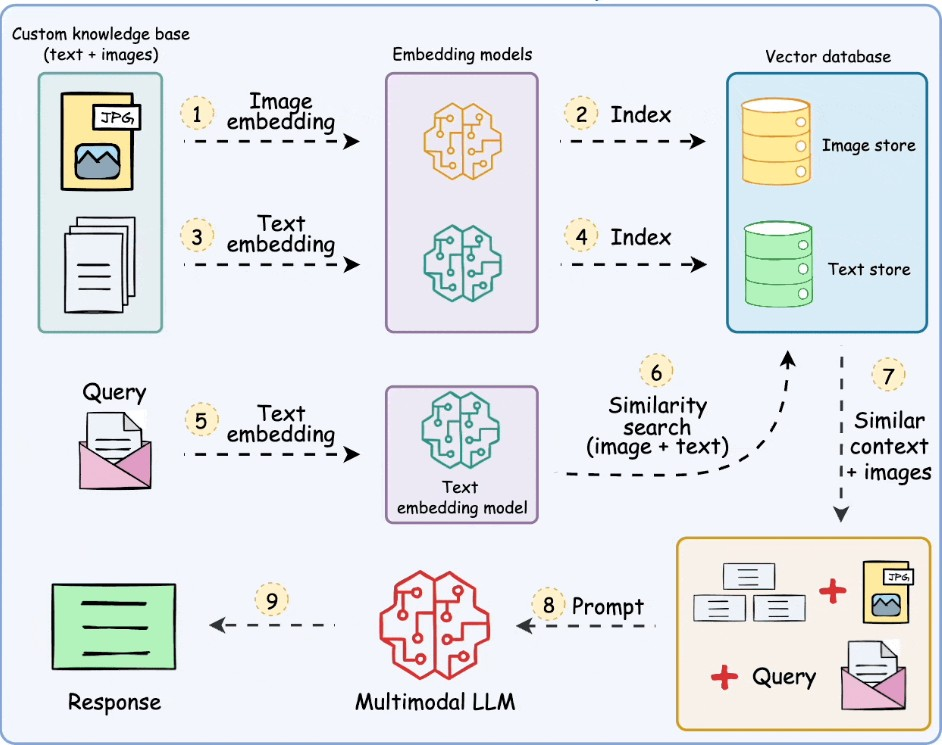
\includegraphics[width=0.8\linewidth,keepaspectratio]{rag62}
		
	
		% \end{center}

% {\tiny (Ref: A Crash Course on Building RAG Systems -Daily Dose)}


% \end{frame}

% %%%%%%%%%%%%%%%%%%%%%%%%%%%%%%%%%%%%%%%%%%%%%%%%%%%%%%%%%%%%%%%%%%%%%%%%%%%%%%%%%%
% \begin{frame}[fragile]{Multimodal Embeddings in RAG Workflow}
    % \begin{itemize}
        % \item \textbf{Multimodal Embeddings (e.g., CLIP):} Used for embedding both images and text.
        % \item \textbf{Query/Prompt:} User input initiates the process.
        % \item \textbf{Retrieved Context:} User query retrieves context (images and/or text).
        % \item \textbf{LMM (Language Model):} Context, along with the prompt, passed to the Language Model.
        % \item \textbf{Multimodal Response:} The Language Model generates the final response.
        % \item \textbf{Indexing and RAG Pipelines:} Sequential steps involving embedding, retrieval, and response generation.
    % \end{itemize}
% \end{frame}


% %%%%%%%%%%%%%%%%%%%%%%%%%%%%%%%%%%%%%%%%%%%%%%%%%%%%%%%%%%%
% \begin{frame}[fragile]\frametitle{Multimodal RAG using Multimodal Embeddings}


		% \begin{center}
		% \includegraphics[width=0.6\linewidth,keepaspectratio]{rag12}
		% \end{center}

% {\tiny (Ref: Multimodal RAG - Abhinav  Kimothi)}

% \end{frame}

% %%%%%%%%%%%%%%%%%%%%%%%%%%%%%%%%%%%%%%%%%%%%%%%%%%%%%%%%%%%
% \begin{frame}[fragile]\frametitle{CLIP : Contrastive Language-Image Pre-training}


		% \begin{center}
		% \includegraphics[width=0.6\linewidth,keepaspectratio]{rag13}
		% \end{center}

% {\tiny (Ref: Multimodal RAG - Abhinav  Kimothi)}

% \end{frame}


% %%%%%%%%%%%%%%%%%%%%%%%%%%%%%%%%%%%%%%%%%%%%%%%%%%%%%%%%%%%%%%%%%%%%%%%%%%%%%%%%%%
% \begin{frame}[fragile]{MM-RAG Paper and Implementations}
    % \begin{itemize}
        % \item MM-RAG paper published in June 2023 provides insights into building a retriever for multimodal RAG.
        % \item LangChain cookbook offers a simple implementation of multimodal RAG using a multiquery retriever and OpenAI GPT4V.
        % \item LlamaIndex tutorial explains multimodal RAG implementation in detail.
    % \end{itemize}
% \end{frame}

% %%%%%%%%%%%%%%%%%%%%%%%%%%%%%%%%%%%%%%%%%%%%%%%%%%%%%%%%%%%%%%%%%%%%%%%%%%%%%%%%%%
% \begin{frame}[fragile]{Using LMMs for Text Summaries from Images}
    % \begin{itemize}
        % \item \textbf{Indexing:}
            % \begin{itemize}
                % \item LLM generates captions for images in the data.
                % \item Captions and text summaries stored as text embeddings in a vector database.
                % \item Maintains a mapping from image captions to image files.
            % \end{itemize}
        % \item \textbf{Generation:}
            % \begin{itemize}
                % \item User query with text and image.
                % \item LLM generates image captions and embeddings.
                % \item Search for text summaries and image captions; retrieve images based on relevant captions.
                % \item Retrieved content passed to LMM with a prompt.
                % \item LMM generates a multimodal response.
            % \end{itemize}
    % \end{itemize}
% \end{frame}

% %%%%%%%%%%%%%%%%%%%%%%%%%%%%%%%%%%%%%%%%%%%%%%%%%%%%%%%%%%%
% \begin{frame}[fragile]{Using LMMs for Text Summaries from Images}


		% \begin{center}
		% \includegraphics[width=0.6\linewidth,keepaspectratio]{rag14}
		% \end{center}

% {\tiny (Ref: Multimodal RAG - Abhinav  Kimothi)}

% \end{frame}


%%%%%%%%%%%%%%%%%%%%%%%%%%%%%%%%%%%%%%%%%%%%%%%%%%%%%%%%%%%%%%%%%%%%%%%%%%%%%%%%%%
\begin{frame}[fragile]\frametitle{}
\begin{center}
{\Large Chunking}

{\tiny (Ref: Mastering RAG: Advanced Chunking Techniques - Pratik Bhavsar)}

\end{center}
\end{frame}

%%%%%%%%%%%%%%%%%%%%%%%%%%%%%%%%%%%%%%%%%%%%%%%%%%%%%%%%%%%
\begin{frame}[fragile]\frametitle{What is Chunking?}
      \begin{itemize}
\item Breaking down texts into smaller, manageable pieces called "chunks"
\item Each chunk becomes a vectorized unit of information stored in database
\item Fundamentally shapes efficiency and effectiveness of NLP tasks
\item Central role in RAG systems affecting both retrieval and response quality
\item Creates the foundation for information retrieval in vector databases
\item Essential preprocessing step for LLM applications
  \end{itemize}

\end{frame}

%%%%%%%%%%%%%%%%%%%%%%%%%%%%%%%%%%%%%%%%%%%%%%%%%%%%%%%%%%%
\begin{frame}[fragile]\frametitle{What is Chunking?}

  
  	\begin{center}
	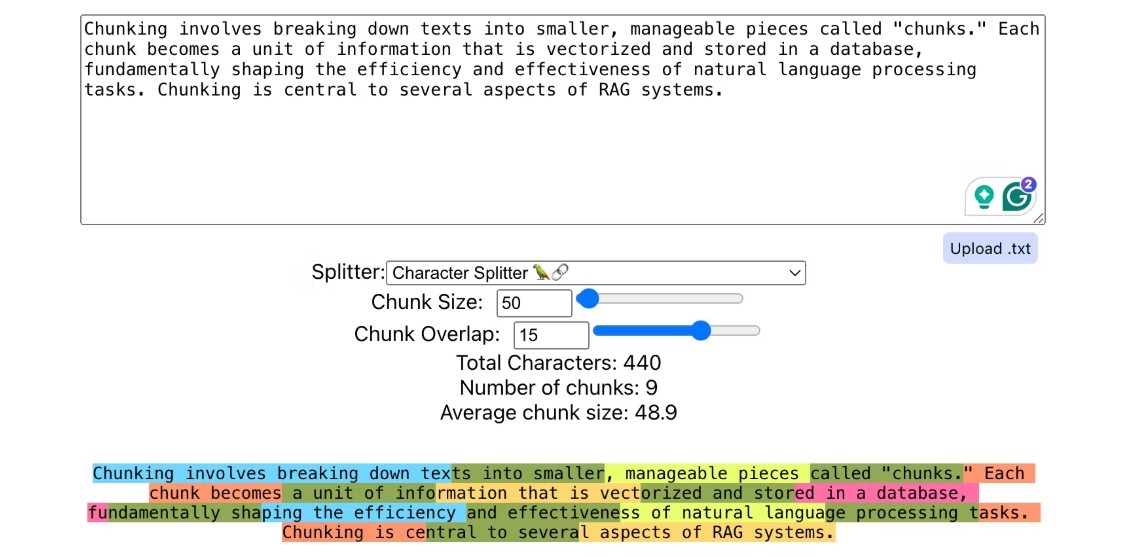
\includegraphics[width=\linewidth,keepaspectratio]{rag72}
	
	{\tiny (Ref: Mastering RAG: Advanced Chunking Techniques - Pratik Bhavsar)}
	
	\end{center}
\end{frame}

%%%%%%%%%%%%%%%%%%%%%%%%%%%%%%%%%%%%%%%%%%%%%%%%%%%%%%%%%%%
\begin{frame}[fragile]\frametitle{Impact of Chunking on RAG Systems}
      \begin{itemize}
\item \textbf{Retrieval Quality}: Defines unit of information stored, enables retrieval of most relevant content
\item \textbf{Vector Database Cost}: Storage costs grow linearly with number of chunks
\item \textbf{Query Latency}: Fewer chunks reduce latency for real-time applications
\item \textbf{LLM Costs}: Larger chunks increase serving costs and latency
\item \textbf{Hallucination Control}: Excessive context can lead to LLM hallucinations
\item \textbf{Balance Required}: Must optimize between contextual richness and retrieval precision
  \end{itemize}
\end{frame}

%%%%%%%%%%%%%%%%%%%%%%%%%%%%%%%%%%%%%%%%%%%%%%%%%%%%%%%%%%%
\begin{frame}[fragile]\frametitle{Key Factors Influencing Chunking Strategy}
      \begin{itemize}
\item \textbf{Text Structure}: Content type (sentences, paragraphs, code, tables) affects chunk size
\item \textbf{Embedding Model}: Model capabilities and context length limitations guide strategy
\item \textbf{LLM Context Window}: Finite context windows constrain chunk size decisions
\item \textbf{Question Types}: Factual vs complex questions require different approaches
\item \textbf{Application Needs}: No one-size-fits-all solution exists
\item \textbf{Performance Trade-offs}: Must balance multiple competing factors
  \end{itemize}
\end{frame}

%%%%%%%%%%%%%%%%%%%%%%%%%%%%%%%%%%%%%%%%%%%%%%%%%%%%%%%%%%%
\begin{frame}[fragile]\frametitle{What is Chunking?}

  
  	\begin{center}
	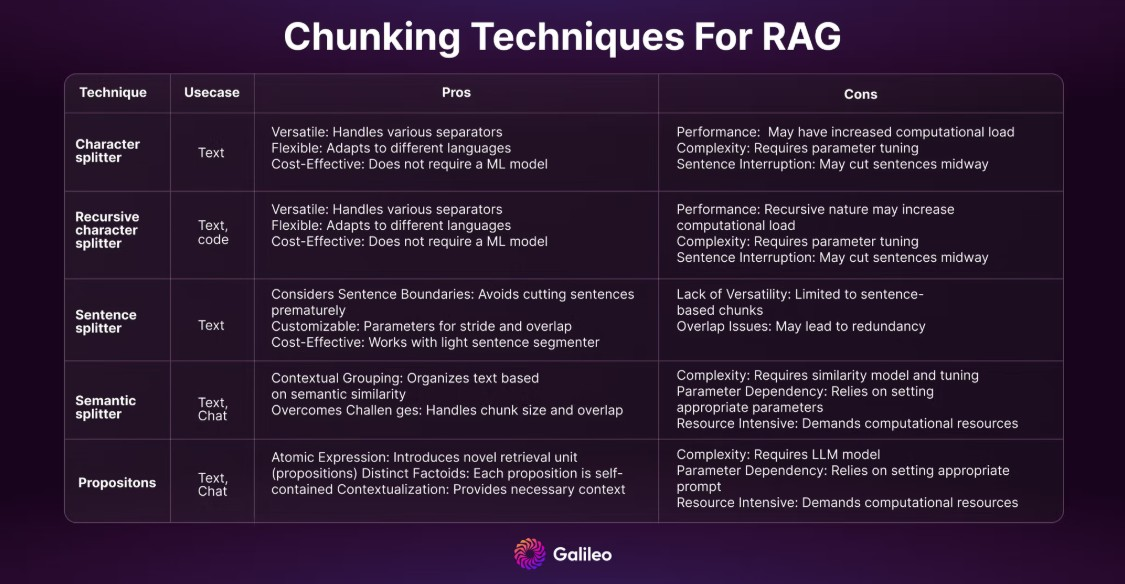
\includegraphics[width=\linewidth,keepaspectratio]{rag73}
	
	{\tiny (Ref: Mastering RAG: Advanced Chunking Techniques - Pratik Bhavsar)}
	
	\end{center}
\end{frame}

%%%%%%%%%%%%%%%%%%%%%%%%%%%%%%%%%%%%%%%%%%%%%%%%%%%%%%%%%%%
\begin{frame}[fragile]\frametitle{Text splitter}

  
  	\begin{center}
	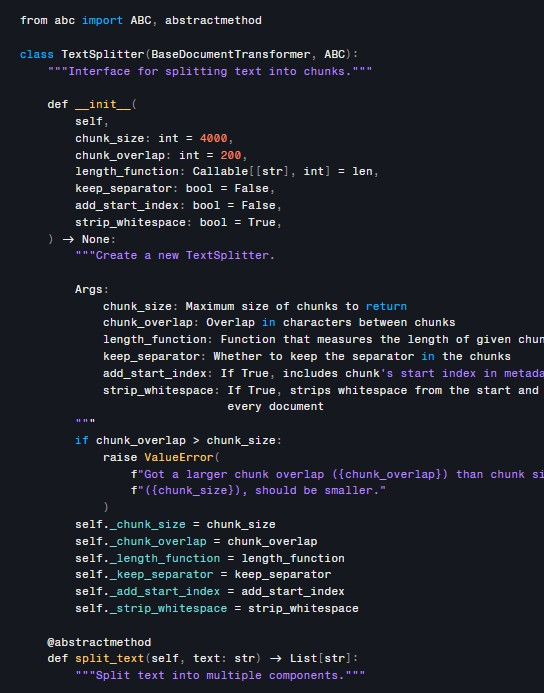
\includegraphics[width=0.45\linewidth,keepaspectratio]{rag74}
	
	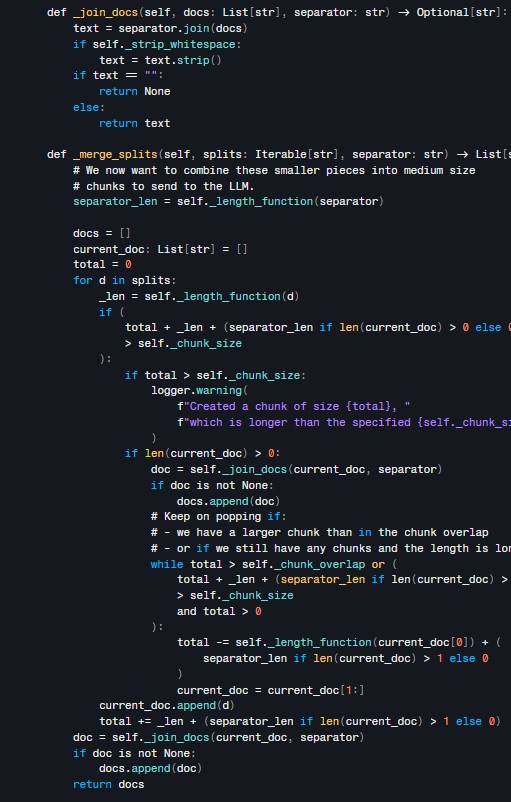
\includegraphics[width=0.45\linewidth,keepaspectratio]{rag75}
	
	{\tiny (Ref: Mastering RAG: Advanced Chunking Techniques - Pratik Bhavsar)}
	
	\end{center}
\end{frame}

%%%%%%%%%%%%%%%%%%%%%%%%%%%%%%%%%%%%%%%%%%%%%%%%%%%%%%%%%%%
\begin{frame}[fragile]\frametitle{Character Splitter Technique}
      \begin{itemize}
\item Uses separator (e.g., "\textbackslash n") to identify text split points
\item Merges splits into chunks based on chunk\_size and chunk\_overlap parameters
\item Simple approach but can cut sentences midway
\item Example: Empty string separator treats each character as splitter
\item Combines splits according to specified size constraints
\item Foundation for more sophisticated splitting methods
  \end{itemize}
\end{frame}

%%%%%%%%%%%%%%%%%%%%%%%%%%%%%%%%%%%%%%%%%%%%%%%%%%%%%%%%%%%
\begin{frame}[fragile]\frametitle{Character splitter}

  
  	\begin{center}
	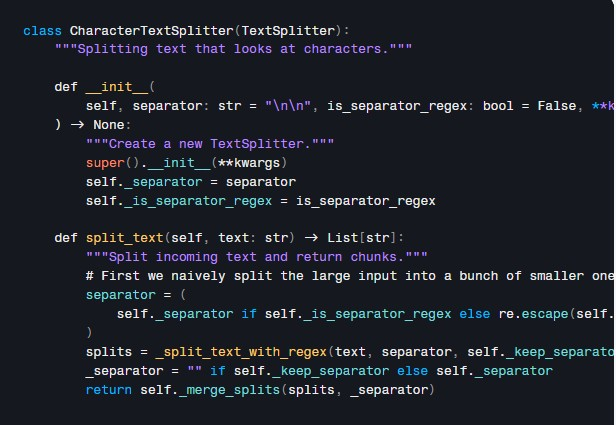
\includegraphics[width=0.45\linewidth,keepaspectratio]{rag76}
	
	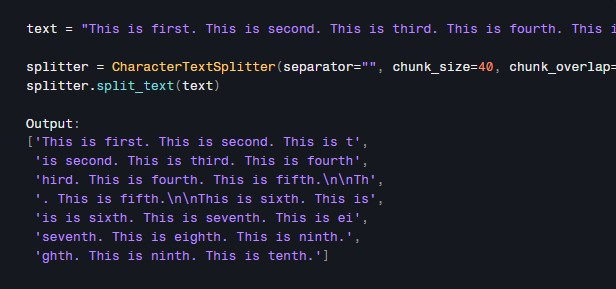
\includegraphics[width=0.45\linewidth,keepaspectratio]{rag77}
	
	{\tiny (Ref: Mastering RAG: Advanced Chunking Techniques - Pratik Bhavsar)}
	
	\end{center}
\end{frame}

%%%%%%%%%%%%%%%%%%%%%%%%%%%%%%%%%%%%%%%%%%%%%%%%%%%%%%%%%%%
\begin{frame}[fragile]\frametitle{Recursive Character Splitter}
      \begin{itemize}
\item Recursively attempts splitting using different separators
\item Uses hierarchical list of separators in order of preference
\item For Python: tries class definitions, function definitions, then common patterns
\item More flexible and adaptive than simple character splitting
\item Processes text recursively until manageable chunk sizes achieved
\item Language-specific separators available for code chunking
  \end{itemize}
\end{frame}

%%%%%%%%%%%%%%%%%%%%%%%%%%%%%%%%%%%%%%%%%%%%%%%%%%%%%%%%%%%
\begin{frame}[fragile]\frametitle{Sentence Splitter Approach}
      \begin{itemize}
\item Uses SpaCy library to identify sentence boundaries
\item Divides text into chunks containing specific number of sentences
\item Controls chunk size with stride and overlap parameters
\item Avoids cutting sentences midway (major advantage over character splitting)
\item Maintains sentence integrity and readability
\item Still faces challenges with pronoun references requiring context
  \end{itemize}
\end{frame}

%%%%%%%%%%%%%%%%%%%%%%%%%%%%%%%%%%%%%%%%%%%%%%%%%%%%%%%%%%%
\begin{frame}[fragile]\frametitle{Semantic Splitting - The Favorite Method}
      \begin{itemize}
\item Groups sentences based on semantic similarity using embedding models
\item Measures similarity between neighboring sentences
\item Creates coherent groups where sentences are contextually related
\item Handles coreference resolution (e.g., pronouns like "they")
\item Overcomes chunk size and overlap management challenges
\item Produces more meaningful and contextually coherent chunks
  \end{itemize}
\end{frame}

%%%%%%%%%%%%%%%%%%%%%%%%%%%%%%%%%%%%%%%%%%%%%%%%%%%%%%%%%%%
\begin{frame}[fragile]\frametitle{LLM-Based Chunking: Propositions}
      \begin{itemize}
\item Novel approach using "propositions" as atomic expressions of meaning
\item Each proposition represents distinct, self-contained factoid
\item Three principles: distinct meaning, minimal/indivisible, self-contained with context
\item Performs automatic coreference resolution
\item Uses specialized propositionizer models (e.g., chentong00/propositionizer-wiki-flan-t5-large)
\item Produces self-sufficient sentences with resolved references
  \end{itemize}
\end{frame}

%%%%%%%%%%%%%%%%%%%%%%%%%%%%%%%%%%%%%%%%%%%%%%%%%%%%%%%%%%%
\begin{frame}[fragile]\frametitle{Multi-Vector Indexing Strategies}
      \begin{itemize}
\item \textbf{Smaller Chunks}: Divide documents into smaller pieces (ParentDocumentRetriever)
\item \textbf{Summary Approach}: Generate and embed document summaries
\item \textbf{Hypothetical Questions}: Create questions each document could answer
\item Indexes both generated content and original text
\item Improves recall of retrieval system
\item Utilizes text2text models or LLMs with prompts for chunk generation
  \end{itemize}
\end{frame}

%%%%%%%%%%%%%%%%%%%%%%%%%%%%%%%%%%%%%%%%%%%%%%%%%%%%%%%%%%%
\begin{frame}[fragile]\frametitle{Document-Specific Splitting with Unstructured}
      \begin{itemize}
\item Handles complex documents with tables, images, and varied formatting
\item Supports major document types: PDF, DOCX, PPTX, XLSX, HTML, XML, images
\item Adaptive partitioning with "auto" strategy for optimal processing
\item Specialized strategies: "fast" (NLP), "hi\_res" (detectron2), "ocr\_only" (OCR)
\item Extracts structured elements: titles, tables, images, headers, footers
\item Enables tabular QnA through HTML table generation
  \end{itemize}
\end{frame}

%%%%%%%%%%%%%%%%%%%%%%%%%%%%%%%%%%%%%%%%%%%%%%%%%%%%%%%%%%%
\begin{frame}[fragile]\frametitle{Measuring Chunking Effectiveness}
      \begin{itemize}
\item \textbf{Chunk Attribution}: Binary metric determining if chunk influenced model response
\item \textbf{Chunk Utilization}: Measures fraction of chunk text impacting response (0-1 scale)
\item Attribution identifies chunks affecting response for troubleshooting
\item Low utilization suggests chunks may be longer than necessary
\item Helps optimize number of retrieved chunks for efficiency
\item Enables faster debugging and system improvement
  \end{itemize}
\end{frame}

%%%%%%%%%%%%%%%%%%%%%%%%%%%%%%%%%%%%%%%%%%%%%%%%%%%%%%%%%%%
\begin{frame}[fragile]\frametitle{Conclusion and Best Practices}
      \begin{itemize}
\item Effective chunking is crucial for optimizing RAG system performance
\item No universal solution - strategy depends on specific use case requirements
\item Consider text structure, embedding model, LLM context, and question types
\item Semantic splitting often provides superior results over character-based methods
\item Use evaluation metrics (Attribution, Utilization) to optimize performance
\item Balance between contextual richness, retrieval precision, and system efficiency
  \end{itemize}
\end{frame}